\section{商品信息提取}
在爬取了一系列京东商品网址之后,我们获得了储存着这些网页URL和处理之后的文件名的文本。

接下来,为获取每件商品的详细信息,我们逐行读取该文本,通过打开每件商品网页的网址,结合beautifulsoup从content内容中截取我们需要的部分,并将其写入用来储存每件商品的具体信息的文本中。注意到京东旗下绝大部分商品网页的html布局都是相似的,我们可以通过定位固定的tag节点,并用“id”、“class”等属性加以限制,从而获取每一个商品网页中同一种商品信息的位置,完成爬取。

例如:我们观察到所有描述商品的图片地址在html中都保存在如图\ref{img:dsw1}所示的“img”标签下的“data-origin”类中,因此我们可以根据这一特点定位图片url的储存位置,利用find\_all()、get()等语句获取信息,并以读写方式将其写入文本文件中。

\begin{figure}[htbp]
\centering
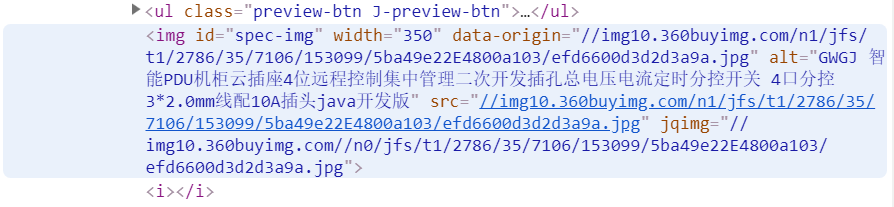
\includegraphics[width=13.5cm]{img/dsw/dsw1.png}
\caption{图片地址的获取}
\label{img:dsw1}
\end{figure}

获取imgurl的代码如下:
\begin{python}
    soup = BeautifulSoup(content,features='html.parser')
    for img in soup.find_all('img', id="spec-img"):
        src = img.get('data-origin', '')
        if (src == '' or not (src.endswith('jpg') or src.endswith('png'))):
            continue
        src = 'http:' + src
        with open(url + '.txt', 'a') as f3:
            f3.write(src)
            print src
            f3.write('\n')
\end{python}

\begin{figure}[htbp]
\centering
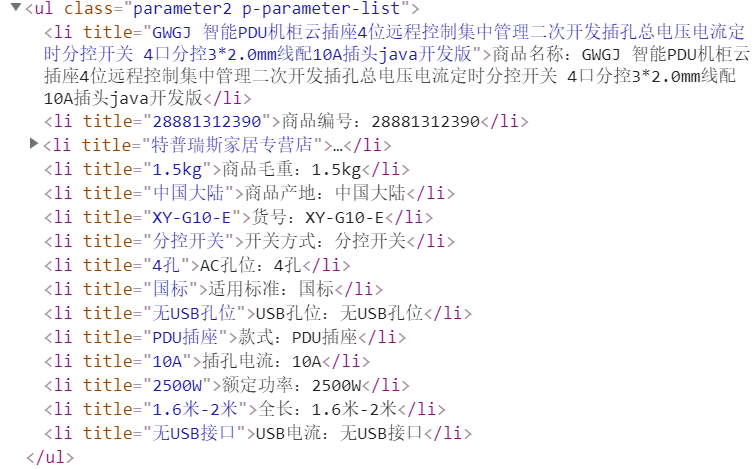
\includegraphics[width=8.5cm]{img/dsw/dsw2.png}
\caption{部分商品信息的获取}
\label{img:dsw2}
\end{figure}

其余商品属性的获取与之类似,比如在“class”为“parameter2 p-parameter-list”的“ul”标签下读取如图\ref{img:dsw2}所示的文本内容,我们可以获得如图\ref{img:dsw3}所示的商品属性:

\begin{figure}[htbp]
\centering
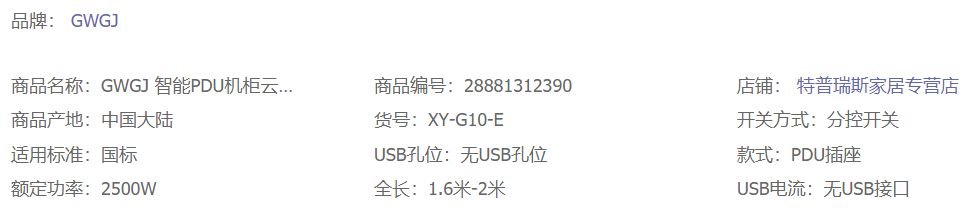
\includegraphics[width=10.5cm]{img/dsw/dsw3.png}
\caption{部分商品信息}
\label{img:dsw3}
\end{figure}

对这部分content进行字符串相关处理操作,就可以得到各项信息,并逐行写入文本中。

需要注意的一项商品属性是商品的价格。如果直接从content中读取价格对应标签下的内容,最终获得的价格就全部为空了。这是由于京东对价格进行了特殊的处理,我们不能像获取其他信息那样直接得到商品价格。在此我通过json获取mgets请求,从而得到了价格。请求语句如下,只保留skuIds这一项参数,其意为商品编号,而该编号可以从content中正常抓取。

\begin{python}
url2 = 'https://p.3.cn/prices/mgets?skuIds=J_' + str(k.contents[3].get('title'))
\end{python}

通过改变代码中的商品编号,我们可以得到类似于图\ref{img:dsw4}的响应,其中“p”对应的即为商品价格。(若当前商品已经下架,则“p” 值为-1)因此我们只需要获取该页面的文本,并定位到“p”字符后的数字即为价格。

\begin{figure}[htbp]
\centering
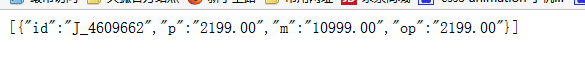
\includegraphics[width=11.5cm]{img/dsw/dsw4.png}
\caption{京东商品价格的获取}
\label{img:dsw4}
\end{figure}

当一件商品的相关detail全部被获取并储存之后,得到的文本如图\ref{img:dsw5}所示:共八行信息,从上到下依次为商品概述、网页URL、图片URL、商品名、品牌、价格、商品类别、其他属性。

\begin{figure}[htbp]
\centering
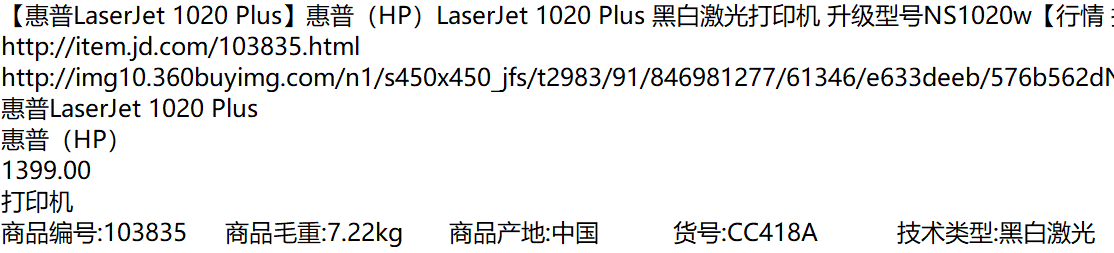
\includegraphics[width=12.5cm]{img/dsw/dsw5.png}
\caption{京东商品detail的保存}
\label{img:dsw5}
\end{figure}

至此,获取商品detail的部分就实现了。以上过程的实现代码保存在getdetail.py文件中。